\documentclass[12pt]{report}
\usepackage[utf8]{inputenc}
\usepackage[english]{babel}
\usepackage{appendix}
\usepackage{graphicx}
\graphicspath{{assets/}}
\usepackage[a4paper,top=25mm,bottom=30mm,width=140mm]{geometry}
\usepackage{pdflscape}
\usepackage{afterpage}
\usepackage{float}
\setcounter{tocdepth}{0}
\newcommand\tab[1][0.75cm]{\hspace*{#1}}

\newcommand\blankpage{%
    \null
    \thispagestyle{empty}%
    \addtocounter{page}{-1}%
    \newpage}

\usepackage{fancyhdr}
\pagestyle{fancy}
\fancyhead{}
\fancyhead[C]{\leftmark}
\renewcommand{\headrulewidth}{0.4pt}

\usepackage[]{algorithm2e}

%\usepackage{listings}
\usepackage[nottoc]{tocbibind}
\usepackage{url}
\usepackage[some]{background}

\SetBgScale{1}
\SetBgContents{\parbox{10cm}{%
    \Huge Draft:  \today\\[14cm]\rotatebox{180}{\Huge Draft:  \today}}}
\SetBgColor{gray}
\SetBgAngle{270}
\SetBgOpacity{0.2}

\begin{document}
\begin{titlepage}
    \newgeometry{width=150mm,top=40mm,bottom=40mm}
    \begin{center}
        \vspace*{1cm}
        Department of Computing\\
        Goldsmiths, University of London\\

        \vspace*{3.25cm}

        \textbf{\LARGE Augmented Reality Navigation System\\}
        \vspace*{0.20cm}           
        \textbf{\LARGE for Commercial Spaces}\\
        \vspace*{0.55cm}           
        {\large Proposal}\\
        \vspace*{0.15cm}           

        \vspace*{2cm}
        by\\
        \vspace*{0.25cm}   

        \textbf{Arif Kharoti, Nicholas Orford-Williams, Hardik Ramesh,\\}
        \textbf{Gabriel Sampaio Da Silva Diogo, Hamza Sheikh, Jonathan Tang\\}
        \vspace*{0.1cm}    
        Software Projects – Group 14\\  

        \vspace{2cm}

        Autumn 2018
        \vfill

        Submitted in partial fulfillment for the degree of\\
        \textit{Bachelor of Science} in \textit{Computer Science}

        \vspace{1.5cm}

    \end{center}
\end{titlepage}

\afterpage{\blankpage}
\thispagestyle{plain}

\pagenumbering{roman}

\newgeometry{top=25mm,bottom=30mm,width=140mm}
\begin{center}        
    \large
    \textbf{Abstract}\\
\end{center}

% Rewrite this section
% The LAST thing to write
Frustration and confusion are common emotions that are apparent at large shopping centres. After analysing recent studies, it is evident that shopping centres have a huge role to play in the overall retail experience. In order to provide greater value to both consumers and retailers, retail settings are being challenged to become smarter. One approach that is becoming increasingly recognised is mobile augmented reality (MAR) apps. Many consumers have difficulties in locating the store which satisfies their needs. In this research, we endeavour to outline the market requirement of developing an application that allows for smart retail and describing how additional value is created to customers as well as benefiting retailers. It is proposed that the application will implement a 3D model of various shopping centres, featuring navigation functionality to assist users in finding their desired store.\\

\vspace*{1.5cm}

\begin{center}    
    \large
    \textbf{Word Count}\\
    xyz\\
    \normalsize computed by \texttt{TeXcount}
\end{center}

\tableofcontents
\afterpage{\blankpage}

\chapter{Concept Introduction \& User Needs}
\pagenumbering{arabic}
% This should explain your project idea. You can presume that the reader has a basic level of technical knowledge but not specific knowledge of your particular area, so communicate your ideas clearly.

The main concept for this project revolves around the use of augmented reality (AR) navigation on smartphones. AR is the superimposing of a computer-generated image onto a user's view of the real world \cite{oxforddict}. This technology first came about in the 1960s \cite{InteractionDesign} but has recently gained wide-spread consumer and media attention after the use of on Snapchat filters \cite{Snapchat} and the 2016 game \textit{Pokémon Go} for example. There have been many times where people get lost in unfamiliar spaces such as a museum, immersed by the culture around them, and their sense of direction. This project aims to tackle this issue by allowing users to restore their orientation by having a mobile platform to route users to their destination, using AR. The platform will use the device's camera to work out its surrounding, and will produce a highlighted line on the screen to their destination in real time.\\

This concept has various applications to other similar scenarios such as finding products in a supermarket, books in a library, or even valuable items that people own that can emit an electronic signal for it to be tracked down. Further, the concept could also use machine learning in identifying user's traits in places visited in a museum in order to give personalised recommendations at other similar exhibitions.



\chapter{Stakeholder Requirements}
% You should identify the stakeholders of any software you are developing and reason that they have an interest in your concept.

After consulting with the main stakeholders are museum visitors and staff, and potential users of the proposed application, a better understanding was available, concerning the apparent need that was in the relative market regarding museums. Out of the 21 responses received, 15 potential users admitted to visiting museums at least once a month; showing some level of frequency in their visits, and that something can be offered to this group of people.\\

Since the concept principally considers the use of navigation in museums, when users were asked, "do you find yourself using the maps in the museum more than once?"- 100\% of visitors agreed that they referred to the maps around the museum multiple times, and some respondents over 10 times. However, these maps are not free; in most museums, including the Natural History Museum and the Science Museum in London, require a fee of £1.\\

18 of the respondents agreed they preferred using their phone to navigate rather than the paper maps. Outlining a clear need for an accessible tool other than the maps around the museum.\\

Based on the stakeholder research, the project requirements are, 

\begin{itemize}
    \item navigate the user to a museum through the use of augmented reality
    \item to display navigational routes in real time
    \item calculate the shortest route to the user specified location 
    \item work transferrably in other museums/commercial spaces
    \item contain accessibility features such as magnified text and inverted colours for example
\end{itemize}

Another key stakeholder are museum staff as they are instrumental to any on-the-ground assistance in terms of navigation. Furthermore, the application should endeavour to make it easier for museum staff to assist visitors.\\

The stakeholder requirements of museum staff are,

\begin{itemize}
    \item Exhibit an effective and easy-to-use design. 
    \item Be economic and effective in its use of data, as most data would be sourced from the museum Wi-Fi. 
    \item Written content and other media to be within control of the museum.
\end{itemize}

During the field research, museum-floor staff and receptionists were also consulted. The staff approached had all received a navigational inquiry, either from themselves or visitors. Although positive responses were received several concerns were cited,\\

\begin{itemize}
    \item Battery performance
    \item Data usage
    \item Ease of use
\end{itemize}

\chapter{Prior Knowledge}
% You should describe how you gathered relevant information for credible sources, summarised and analysed that data, and how that information altered the proposed concept. 
% Computer Science: you should explain the computer science problems presented by your project, satisfying the programme learning outcome “Apply computational thinking to the design and implementation of moderately complex computing systems”.

\section{Current Solutions \& Competitors}
The market of indoor museum navigation has grown recently with more solutions being submitted due to the growth in indoor navigational research. Most solutions cater well for a basic navigation of large public spaces, but fail to display an even proportion of navigational, and interactive content with well-presented data.\\

Since most museums use portable audio guides, user experiences can be vastly improved by mobile devices. Currently only a few solutions can be found; the Orpheo group \cite{orpheo} provide a unique app for each place; their solution is cumbersome to regular museumgoers who wish to have a hassle-free setup. As the aim is to appeal to museums, having an application whereby the user can walk into a museum, and greeted with relevant information is vital in comparison \cite{microsoft}.\\

If museums wanted a solution for navigation, due to the low number of museum-specific competitors, would choose to use a standard indoor mapping software \cite{engadget}. However, while there are many options out there from Google and Mapspeople \cite{mapspeople} who try to provide this, they lack exigencies that are imperative for museums like heavily-integrated AR, and intelligent tour guiding from your location.\\ 
% and virtual reality to take a scene from the museum, for instance, and place the user to the artefact's original time and place.\\

From a technological viewpoint, a problem in the solutions that museums implement today, would be their paper maps not processing real-time locations. AR allows for real-time data processing, picking up the user's current location, and displaying the best route for the user to take through their device's camera. A benefit of implementing AR is the unique approach to today's navigation solutions, whilst allowing users to create their own content, enabling more opportunities to interact with the application.

\chapter{Design}
\documentclass{article}
\usepackage[utf8]{inputenc}
\usepackage{graphicx}
\usepackage{float}

\author{Hamza Sheikh}

\begin{document}

\subsection{The Importance of Design}

Design is a great initial investment owing to a number of different reasons. Having a design process allows for more efficiency and transparency when actually coming to design the application. It overcomes the risk of having to refer back to the drawing board when actually developing the application, setting in stone the main features and functionality of the application.\\

\subsection{The Unified Modeling Language}

A way in which effective design strategies were carried out was through the implementation of the Unified Modeling Language (UML), a powerful standard for creating specifications of various parts of a software system.\\

\\One example of the UML was our implementation of a use case diagram which outlined the different scenarios in which a user would function the application. See figure~\ref{fig:Use Case Diagram}.\\

\begin{figure}[H]
    \centering
    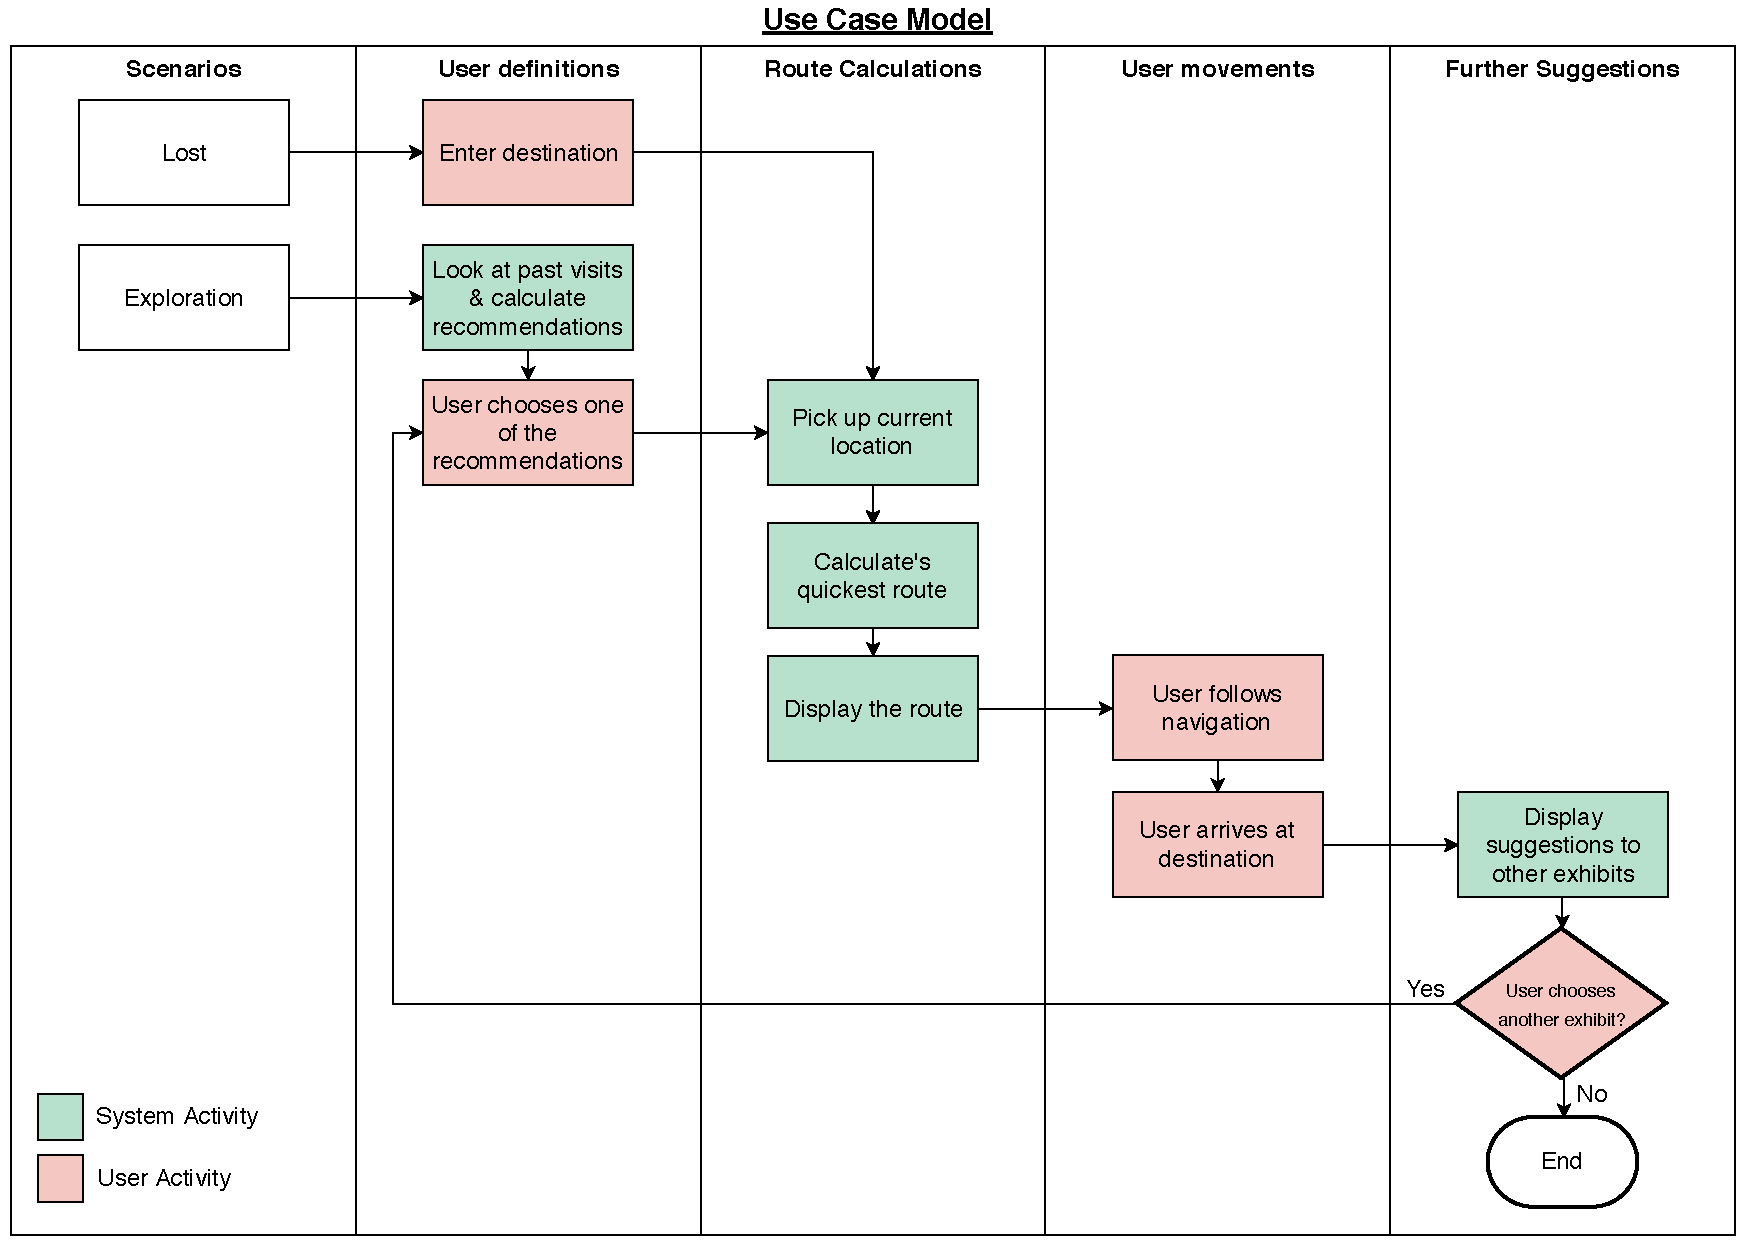
\includegraphics[width=\textwidth]{use_case.pdf}
    \caption{Use Case Diagram}
    \label{fig:Use Case Diagram}
\end{figure}

\\Another way in which UML was implemented to further support and refine the designing phase of the software development was through an activity diagram. (See figure~\ref{fig:Activity Diagram}).

\begin{figure}[H]
    \centering
    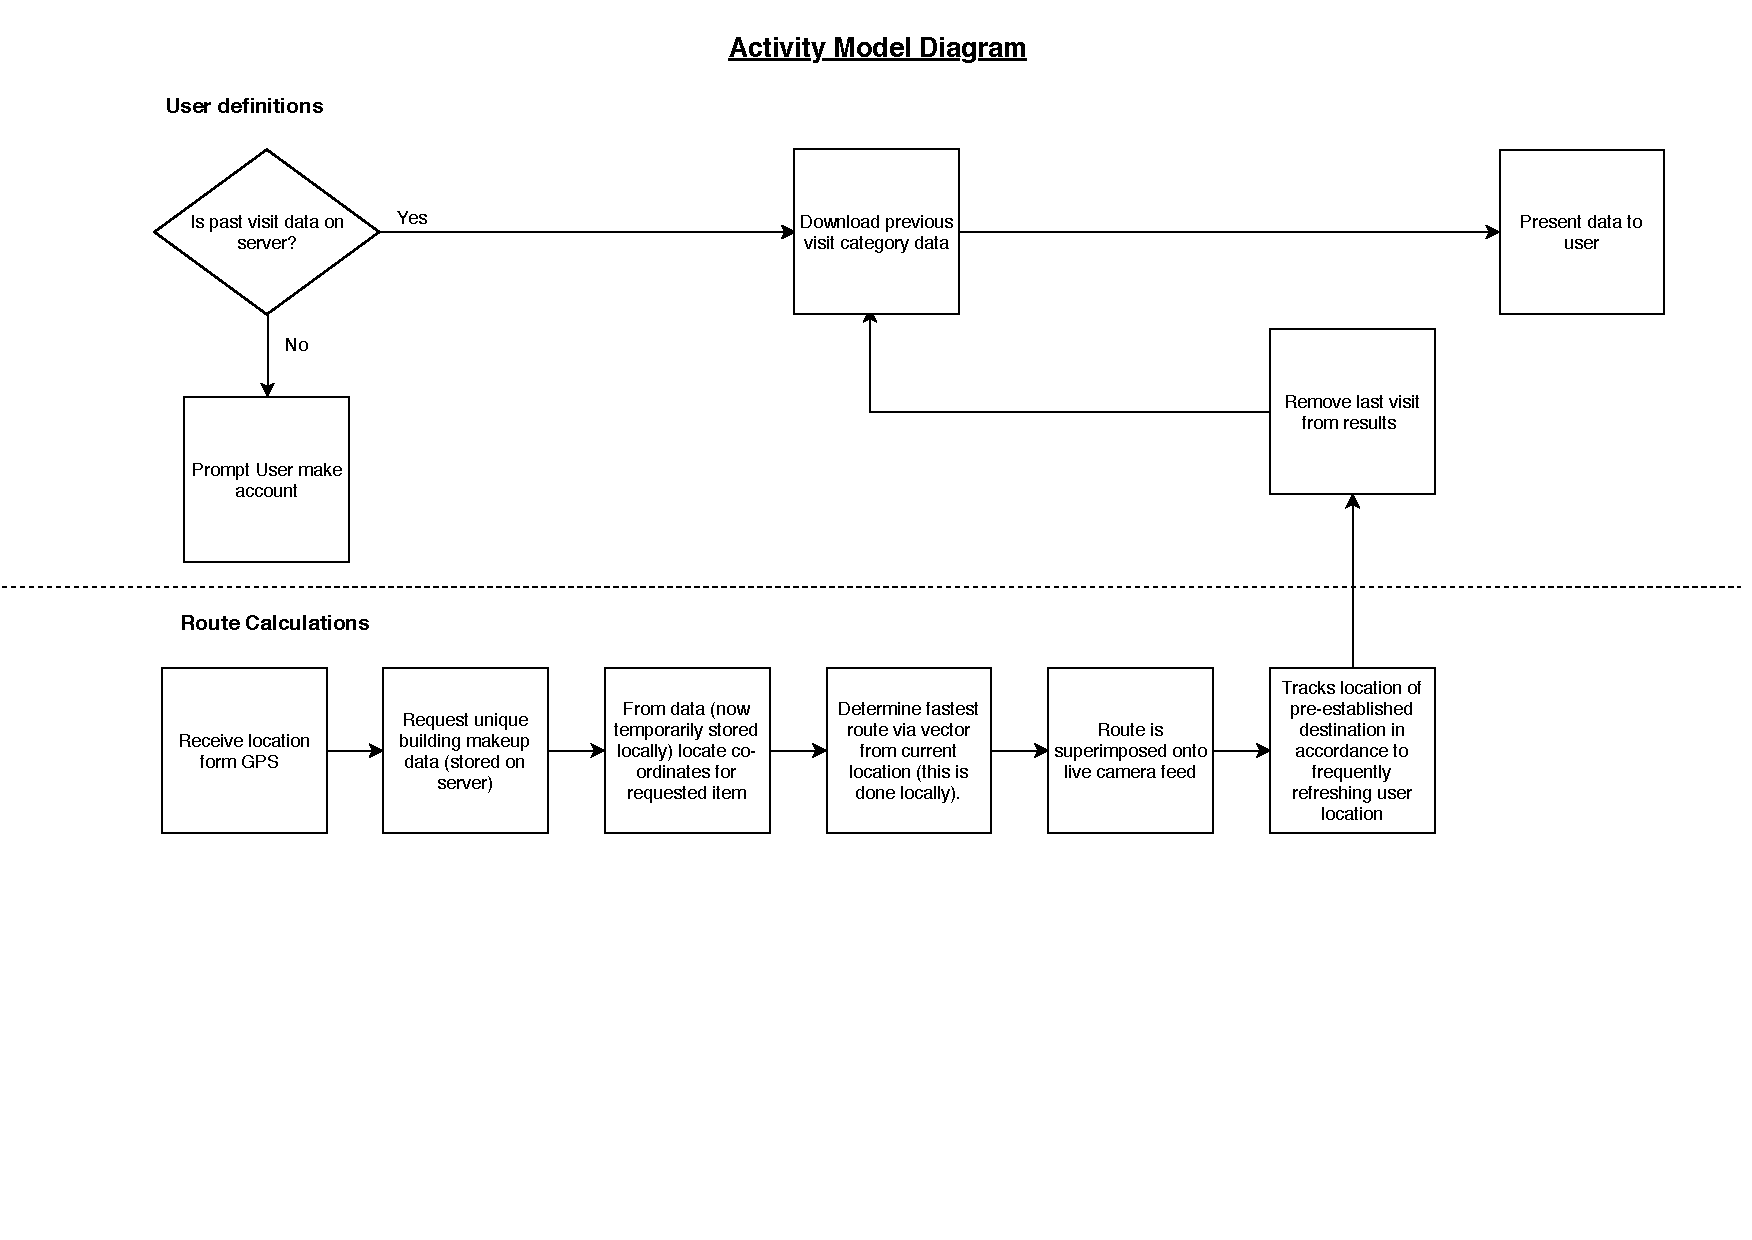
\includegraphics[width=\textwidth]{Activity_Diagram.pdf}
    \caption{Activity Diagram}
    \label{fig:Activity Diagram}
\end{figure}

\\The use case diagram (Figure~\ref{fig:Use Case Diagram}) represents the functional behaviour of the system in terms of goals that can be fulfilled by the system. These goals have been defined in the stakeholder requirements. The activity diagram (Figure~\ref{fig:Activity Diagram}) was designed to model the work flow of the system. One main reason that the activity diagram was essential in the designing phase was that UML included that these diagrams are normally easily comprehensible for both analysts and stakeholders. By producing and creating these models, we were able to have a clear understanding of what the application \textit{has} to do, and enabled us, the developers, to visualise the application for the future.

\subsection{Service Model}

We have to first exclaim that the following cases are born out of one important principle; convenience. The \textbf{'lost'} use case, for example, comes from the fact that the user could be lost for whatever reason. What we would provide through this service would be the quickest and most \textbf{convenient} solution to finding their destination. Whether that be the exit, a cafe or a particular exhibition. Another use case;
\textbf{'exploration'}, would become more convenient with the museum, and all its exhibitions (along with brief descriptions) at your fingertips (instead of the existing navigation options present at museums today e.g. wall-maps or paper maps).
\subsubsection*{Model around two cases (The lost and the exploring) }
The lost-case and exploration-case has a virtually linear-stream of logic, and is as follows:
\begin{enumerate}
    \item The user enters within the radius of an environment modelled by the service. In this case, a museum.
    \item The user’s location is picked up once they give use permission to (in this case, it would typically be when the user opens the app). 
    \item The user then picks their destination.
    \item That location is then taken and parsed through a function containing an algorithm that calculates the most convenient route between the user’s real-time location and their desired destination.
    \item The user is then displayed the route, and directed towards their destination via their camera.
    \item Once done, the user is given curated suggestions on possible places they can go.
\end{enumerate}

\end{document}


\chapter{Prototyping}
% Describe the prototyping you did, and what you learned from this, particularly the low fidelity interaction prototypes, any technical prototypes to explore technical feasibility of the solution, and the functional digital prototypes that you used with users to validate that what you are developing meets the expectations of users.

\section{Augmented Reality Libraries}
In order to identify libraries that are good for implementing AR on mobile devices, we divided this prototyping into three platforms to explore them, and built test applications to find out how they help with the project.

\subsection*{Vulforia (Unity/Android)}
Unity is a cross-platform game engine, used to test a simple AR camera prototype where the device's camera hovers an object/image, and displaying information about that object/image on the device. The application was built using Vuforia, an SDK that enables recognition, and tracking of image targets. This library can be used for the exploration case in the use case model. Although, there is a limited amount of tools for locating user current location compared to Android.

\subsection*{ARKit (iOS)}
A similar prototype to Unity was built on Apple's ARKit using Swift \cite{applear}, which was easy to learn. It was intuitive to implement AR features as there was detailed documentation but logging GPS data was harder compared to Android.

\subsection*{ARCore (Android)}
ARCore was used to create a simple 3D model showing on a mobile device when its camera targets a flat surface. Compared to iOS, it is easier to log GPS location, although connecting the user interface to the scripts was more challenging.

\section{User Interface/User Experience Designs}
The project lends substantial importance to its user interface and experience. As it will be used from a wide cross section of technical ability, the aim for UI will be to make the app as simple, and easy to use as possible without having an impinging effect on any major service the end product will feature. This prerequisite was clearly outlined in the surveying of museum guests and staff alike. Our first mission was to determine what interfaces, and experiences current exists within the museum sector. Many museums did employ simple interfaces but due to their mass-manufacturing, their design felt unoptimized, slow and clunky, with simple barebones media not beyond text and images. Furthermore, this design would fail to deliver anything more complex than texts and images.\\
  
The approach to the UX/UI prototyping was to create a score of different complete interface mockups and exhibit them alongside existing solutions. Three team members independently drew up potential interfaces. These candidates were then put to stakeholders, and all received positive attributes were combined into one.

\chapter{Functional Specification}
% The essential functional elements should be defined and described, including data paths. This functional specification should not assume any specific technologies, only functional technologies (e.g. short range wireless technology is a functional statement whilst Bluetooth is a specific technology)

The main functional elements of our concept are:

\begin{enumerate}
\subsection*{Route Calculation}
    \item Receiving the \textbf{current coordinates} of the user, and the coordinates of the destination will be needed to create the starting and end points for calculating the route. The current location will come from sensors on the user's device, and the destination location will be queried against a mapping system.
    \item The platform can \textbf{calculate the quickest route between two points} specified by the user. Data from the above, and the museum model will be required for this calculation.
% \end{enumerate}

\subsection*{Superimposition}
% \begin{enumerate}
    \item A \textbf{3D line will be superimposed} that navigates the user to their destination. Sensor data from the user's device along with the user's relative position in the model will be required to show the line. Access to the user's camera is essential in this element.
% \end{enumerate}

\subsection*{Suggestion/Reviewal}
% \begin{enumerate}
    \item When the user arrives at their destination, the \textbf{system will give recommendations} based on their current route, and allow the user to rate their journey.
    \item The \textbf{user's camera can recognise artwork/objects}, and will display further information about the piece. There will be a storage area of current pieces in the museum so that the camera can query the information.
\end{enumerate}


\chapter{Ethical Audit}
% You should detail any issues of privacy, data protection or intellectual property rights that may arise, and how you will manage them. You should confirm that you will not be working with minors or vulnerable adults.

AR is currently not heavily regulated in the UK owing to the emergence of this new technology. Areas such as data protection, and intellectual property (IP) need to be strongly considered during the development lifecycle. It should be noted that AR will involve collecting extensive amounts of data per user such as names and address, but also real time location, interactions with other users. Within the scope of this project, we will not be working with minors and vulnerable adults. Since the concept of the project relies on the user's camera, accelerometer, and location data on the user's device, ensuring this data cannot be obtained unlawfully, and fits the scope of the Data Protection Act (1998) along with the EU General Data Protection Regulation (GDPR) is of most importance.\cite{ITProPortal}\\

Based on large virtual reality companies such as Oculus, these obligations are addressed by the form of a privacy policy in order to detail how data is collected, used and if it is shared with third parties. Since GDPR presents many pitfalls for developers, it is critical these regulatory issues are addressed before the completion of the product and not after.\\

Another regulatory standard is the IP of the software. The source code that serves as the underlying foundation of the platform will be be original and qualify for copyright protection. Since computer software is usually excluded from patentability in the UK, any ideas that uses AR producing a technical effect, and its associated hardware can be protected by patents. Based on our competitors, it is important that we do not infringe on their patents owned by third parties. Equally, if the concept makes new technical developments in the AR field, then it should be considered whether it would be eligible for patent protection.\\

% Given that the AR experience is built using a database of information about the real world, the database can be protected by copyright. The concept could take on a machine learning viewpoint by recognising third party logos captured on the user's camera. This could cause an infringement claim since AR could be replicating, replacing trademark or copyright works, or distorting the logo.\\

\chapter{Technical Architecture}
% Having validated the proposed solution with users and answered any open technical or feasibility questions, attribute specific technologies to the functional architecture and present this as a technical architecture. Justify your choice of technologies with reasoned arguments for rejecting or retaining alterative technologies.

\section*{Means of Software Development}    
\underline{\textbf{IDE}} : \underline{Android Studio}
\newline
The \underline{Android Studio} is the only development IDE we'll be utilising because it involves a number of relevant exclusive packages and libraries - that if we were to use other IDEs, would have to be defined and therefore take valuable time from our development of the application itself.
\newline
\newline
\underline{\textbf{Languages}} : \underline{Java \& SQL}
\begin{itemize}
    \item Java is distinctly imperative to the project due to the fact that android app development is almost only possible in this language.
\end{itemize}
\underline{\textbf{Architectural Pattern}} : \underline{MVC (Model-View-Controller)}
\newline
\newline
Our application fits under the MVC pattern perfectly be it that the following are true.
\begin{itemize}
    \item Model = The data provided by the user (example : geolocational data)
    \item View = The front-end interface (example : 3D line to location)
    \item Controller = The algorithms between M\&V (example : route calculation)
\end{itemize}
Along with the fact above, the pattern's simplicity makes the most sensible one we can use.
\newline
\newline
\underline{\textbf{SDKs \& Packages}} : \underline{ARCore}
\begin{itemize}
    \item The ARCore kit by Google gives us the ability to apply the AR element of our application without having to spend time pre-defining AR methods ourselves.
\end{itemize}
\newpage
\section*{Technicalities of satisfying user-related questions and stories}


\chapter{Evaluation Plan}
% How you intend to test and evaluate your software during and after development. It may be useful to specify individual test cases.

\chapter{Project Management}
% How you will manage the development process: milestones, Gantt charts, roles, development methodology etc.
% JT will write this

\chapter{Conclusion}
% Summarise your proposal, including the key points from the previous sections.

\appendix
\chapter{Appendix}
\begin{appendices}
% The appendix or appendices should contain your group meeting minutes and any additional raw material that is referred to in the text (e.g. data from requirements gathering, paper prototypes etc.)
\end{appendices}

%\bibliography
\bibliographystyle{unsrt}
\bibliography{references}

\end{document}
